\documentclass[12pt]{article}

\usepackage{anyfontsize}
\usepackage{enumitem}
\usepackage{physics} 
\usepackage{enumerate}
\usepackage{pgfplots}
\usepackage{pgfplotstable}
\usepackage{tikz,pgfplots}
\usepackage{graphicx}
\usepackage{float} 
\usepackage{subfigure}
\usepackage[toc,page]{appendix}
\usepackage{amsmath}  %I added this so that you can use the align tool for equations!
\usepackage{amssymb}
\usepackage{wasysym} %This package allows you to put emojis in your paper!!!!
%wasysym: \smiley{} \frownie{} see http://milde.users.sourceforge.net/LUCR/Math/mathpackages/wasysym-symbols.pdf for list of most symbols available in this package
\usepackage{array}
\usepackage{tabularx}
\usepackage{cellspace}
\usepackage{geometry}
\usepackage{listings}
\usepackage{color}
\usepackage{fontspec}
\usepackage{booktabs}
\usepackage{newtxtext,newtxmath}
\usepackage{caption}

\makeatletter
  \renewcommand\section{\leftskip 0pt\@startsection {section}{1}{\z@}%
                                    {-3.5ex \@plus -1ex \@minus -.2ex}%
                                    {2.3ex \@plus.2ex}%
                                    {\normalfont\Large\bfseries}}
  \renewcommand\subsection{\leftskip 0pt\@startsection{subsection}{2}{\z@}%
                                      {-3.25ex\@plus -1ex \@minus -.2ex}%
                                      {1.5ex \@plus .2ex}%
                                      {\normalfont\large\bfseries}}
  \newcommand\Xsubsubsection{\@startsection{subsubsection}{3}{\z@}%
                                      {-3.25ex\@plus -1ex \@minus -.2ex}%
                                      {1.5ex \@plus .2ex}%
                                      {\normalfont\normalsize\bfseries\leftskip 3ex}}
  \renewcommand\subsubsection[1]{\Xsubsubsection{#1}\leftskip 3ex}
\makeatother

\geometry{
  a4paper,
  total = {170mm, 257mm},
  left = 20mm,
  top = 20mm,
  }

\definecolor{dkgreen}{rgb}{0,0.6,0}
\definecolor{gray}{rgb}{0.5,0.5,0.5}
\definecolor{mauve}{rgb}{0.58,0,0.82}
\lstset{frame = tb,
        language = Python,
        aboveskip = 3mm,
        belowskip = 3mm,
        showstringspaces = False,
        columns = flexible,
        basicstyle = {\small\ttfamily},
        numbers = left,
        numberstyle = \tiny\color{gray},
        keywordstyle = \color{blue},
        commentstyle = \color{dkgreen},
        stringstyle = \color{mauve},
        breaklines = true,
        breakatwhitespace = true,
        tabsize=4}

\renewcommand\lstlistingname{Algorithm}
\captionsetup[lstlisting]{singlelinecheck=false, margin=12pt, labelsep=default, labelfont=default}
%We can also use: labelsep=period or labelsep=spacce, labelfont=default or labelfont=bf

\pgfplotsset{compat = 1.14}
%%%%%%%%%%%%%%%%%%%%%%%%% Again, Don't change anything Above %%%%%%%%%%%%%%%%%%%%%%%%%

\begin{document}

\title{\textbf{{\normalsize Computational Physics Lab}\\
                Homework 2}}
\author{108000204\\
        Yuan-Yen Peng\\
        Dept.\ of Physics, NTHU\\
        Hsinchu, Taiwan}
\date{\today}
\maketitle

\section{Written Assignments}
  The general second-order ordinary differential equations($x$ depend on time) is 
  \[\ddot{x} + b\dot{x} + cx = g(x)\]
  where $b$, $c$ is the constant, and $g(x)$ is the particular term. We can set the general solution as $x = x_{c} + x_{p}$, where $x_{c}$ is the critical solution; $x_{p}$ is the particular solution.

  \subsection{(a) Normal oscillations}
    \begin{align*}
      &solve\quad m\ddot{x} + kx = 0\\
      &\rightarrow \ddot{x} + \frac{k}{m}x = 0\\
      &set\quad x_{c} = e^{\alpha t - \phi},\quad where\ \phi\ is\ a\ phase,\ depending\ on\ init.\ conds.\\
      &\Rightarrow \alpha^{2}e^{\alpha t - \phi} + \frac{k}{m} e^{\alpha t - \phi} = 0,\quad \alpha = \pm i\sqrt{{\frac{k}{m}}},\quad set\ \omega = \sqrt{{\frac{k}{m}}}\\
      &x = \mathbb{R}(x_{c}) = \cos(\omega t - \phi)\quad \blacksquare
    \end{align*}

  \subsection{(b) Damped oscillations}
    \begin{align*}
      &solve\quad m\ddot{x} + \lambda \dot{x} + kx = 0\\
      &\rightarrow \ddot{x} + \frac{\lambda}{m} \dot{x} + \frac{k}{m}x = 0\\
      &set\quad x_{c} = e^{\alpha t - \phi},\quad where\ \phi\ is\ a\ phase,\ depending\ on\ init.\ conds.\\
      &\Rightarrow \alpha^{2}e^{\alpha t - \phi} + \alpha \frac{\lambda}{m} e^{\alpha t - \phi} + \frac{k}{m} e^{\alpha t - \phi} = 0,\\
      &set\quad \omega_{0} = \sqrt{{\frac{k}{m}}}\ and\quad 2\gamma = \frac{\lambda}{m}\\
      &\Rightarrow \alpha^{2} + 2\gamma \alpha + \omega_{0}^{2} = 0, \quad \alpha_{1,\ 2} = -\gamma \pm \sqrt{\gamma^{2} - \omega_{0}^{2}}\\
      & x = x_{c} = A_1 e^{\alpha_{1}t} + A_2 e^{\alpha_{2}t},\ where\ A_{i}\ depends\ on\ initi.\ conds.\quad \blacksquare
    \end{align*}

  \subsection{(c) Forced oscillations}
  The critical solution of (c), inhomogeneous ODE, is the same as the answer of (b) Hence, we only discuss the particular solution $x_{p}$, which means a stable oscillated solution. The ultimate answer will be $x = x_{c} + x_{p}$.

    \begin{align*}
      &solve\quad m\ddot{x} + \lambda \dot{x} + kx = F_{0}\cos(\omega_f t)\\
      &\rightarrow \ddot{x} + \frac{\lambda}{m} \dot{x} + \frac{k}{m}x = \frac{F_{0}}{m}\cos(\omega_f t)\\
      &set\quad x_{p} = Ae^{i(\alpha t)}\\
      &\Rightarrow -\alpha^{2} A e^{i(\alpha t)} + i \alpha \frac{\lambda}{m} A e^{i(\alpha t)} + \frac{k}{m} A e^{i(\alpha t)} = \frac{F_{0}}{m}\cos(\omega_f t)\\
      &set\quad \omega_{0} = \sqrt{{\frac{k}{m}}}\ and\quad 2\gamma = \frac{\lambda}{m}\\
      &at\ t = 0\ \land use\ the\ stable\ cond.\ \rightarrow \alpha = \omega_{f}\\
      &\Rightarrow A(-\omega_{f}^{2} + 2i\gamma \omega_{f} + \omega_{0}^{2}) = \frac{F_{0}}{m},\quad A = \frac{F_{0} / m}{(\omega_{0}^{2} + 2i\gamma \omega_{f} - \omega_{f}^{2})}\\
      &x_{p} = \mathbb{R}(A e^{i(\alpha t)})
      = \mathbb{R}(\frac{F_{0}}{m} \frac{(\omega_{0}^{2} - \omega_{f}^{2} - 2i\gamma \omega_{f})e^{i\alpha t}}{(\omega_{0}^{2} - \omega_{f}^{2})^{2} + 4\gamma^{2}\omega_{f}^{2}}) 
      = \frac{F_{0} / m}{\sqrt{(\omega_0^{2} - \omega_{f})^{2} + 4\gamma^{2}\omega_{f}^{2}}}\cos(\omega_{f}t - \phi),\\
      &\quad where\ \phi = tan^{-1}(\frac{2\gamma\omega_{f}}{\omega_{f}^{2} - \omega_{0}^{2}})\\
      &\Rightarrow\ x = x_{c} + x_{p}\quad \blacksquare
    \end{align*}

\section{Programming Assignments}
  \subsection{Damped oscillations}
  In this section, we reuse our IVP solver and perform simulations of a damped oscillator (the definition follows the lecture). Make a plot for x and v versus t and a phase diagram (in polar coordinates, u and w)
  \[u = \sqrt{\omega_{0}^2 - \gamma^2}x\]
  \[w = \gamma x + \dot{x}\]
  Additionally, in the class, we have shown that RK4 is the most fitted for the theoretical solution, so we will utilize this as a theoretical reference.

    \subsubsection{(a) Under damping}
    The conditions are
    \[A = 1 [cm],\quad \omega_0 = 1 [rads^{-1}],\quad \gamma = 0.2 [s^{-1}], \quad \phi = -\pi / 2 [rad]\]
    Our results, Figure \ref{2.a.norm} meet our expectations, under damping ($\sqrt{\gamma^{2} - \omega_{0}^{2}} \in \mathbb{R},\quad \gamma^{2} - \omega_{0}^{2}> 0$), with the exponential decay envelope and the trigonometric oscillating solutions of position and velocity. Meanwhile, the polar coordinate will show a spiral, not a circle, due to the dampness and it will evolve from the outer edge to the center where the amplitude is zero. In Figure \ref{2.a.pol}, RK2 behaves more fitted with RK4 rather than the Euler. 

    \begin{figure}[H]
      \centering 
      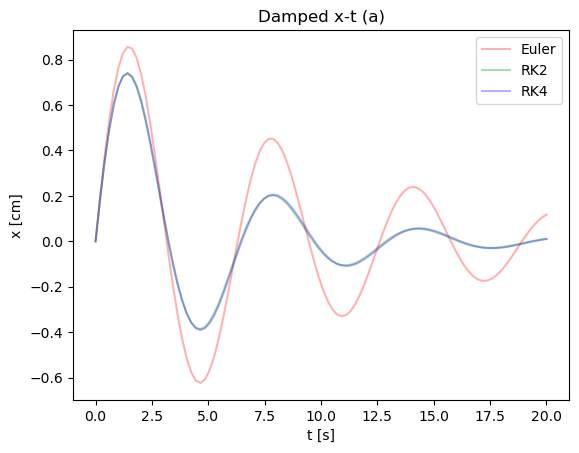
\includegraphics[width = 0.49\textwidth]{damped_a_xt.png}
      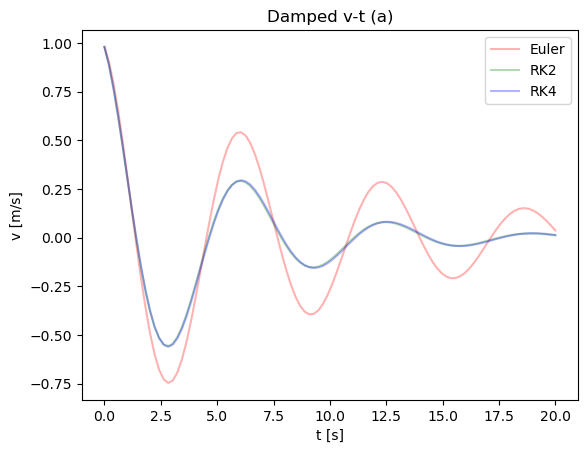
\includegraphics[width = 0.49\textwidth]{damped_a_vt.png}
      \caption{Left is the x-t figure, and right is the v-t. \label{2.a.norm}}
    \end{figure}

    \begin{figure}[H]
        \centering 
        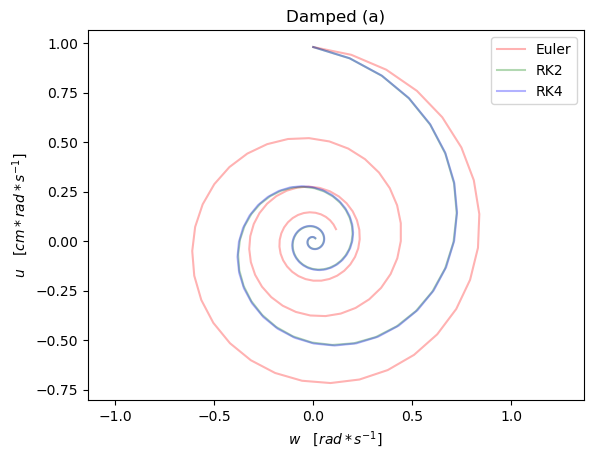
\includegraphics[width = 12cm]{damped_a.png}
        \caption{y-axis is $u$; x-axis is $w$. \label{2.a.pol}}
    \end{figure}

  \subsubsection{(b) Critical damping}
    The conditions are
    \[A = 1 [cm],\quad \omega_0 = 1 [rads^{-1}],\quad \gamma = 1.0 [s^{-1}], \quad \phi = -\pi / 2 [rad]\]
    Our results, this case, $\gamma^{2} = \omega_{0}^{2}$, $\sqrt{\gamma^{2} - \omega_{0}^{2}} = 0$, means ``critical damped''. So as to observe the critical damped figure, we set a very small amplitude instead of 0, and in Figure \ref{2.b.norm}, they meet our expectations. Meanwhile, the polar coordinate will show a straight line, not a spiral, due to the critical condition and it will evolve from the top to the bottom where the amplitude is always zero (indicates that $w = 0$), see in Figure \ref{2.a.pol}. 

    \begin{figure}[H]
      \centering 
      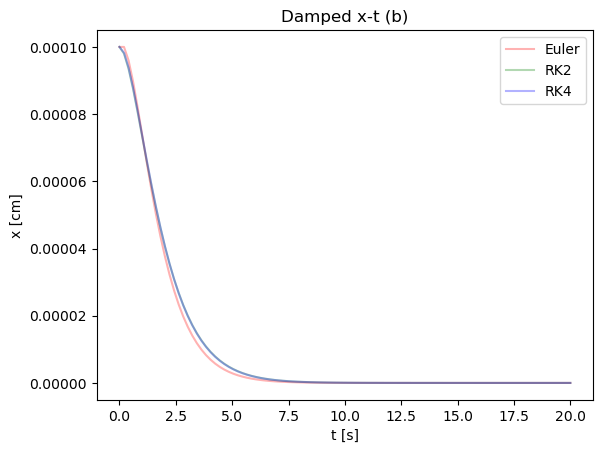
\includegraphics[width = 0.49\textwidth]{damped_b_xt.png}
      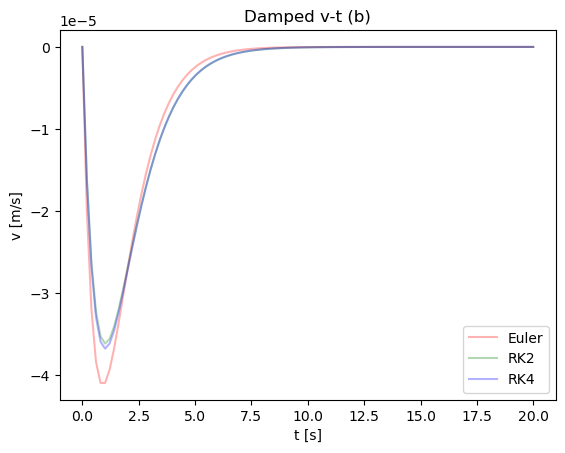
\includegraphics[width = 0.49\textwidth]{damped_b_vt.png}
      \caption{Left is the x-t figure, and right is the v-t. \label{2.b.norm}}
    \end{figure}

    \begin{figure}[H]
        \centering 
        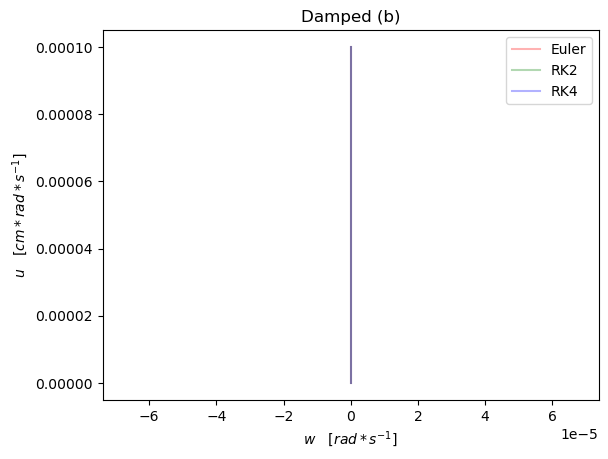
\includegraphics[width = 12cm]{damped_b.png}
        \caption{y-axis is $u$; x-axis is $w$. \label{2.b.pol}}
    \end{figure}

  \subsubsection{(c) Over damping}
    The conditions are
    \[A = 1 [cm],\quad \omega_0 = 1 [rads^{-1}],\quad \gamma = 1.2 [s^{-1}], \quad \phi = -\pi / 2 [rad]\]
    Our results, this case, $\gamma^{2} - \omega_{0}^{2} < 0$, means ``overdamped''.Theoretically, it cannot form a complete period; also with the exponential decay, and in Figure \ref{2.c.norm}, they meet our expectations. Meanwhile, the polar coordinate will show a curve line, not a spiral, due to the overdamped condition and it will evolve from the top to the bottom where the amplitude is positive (indicates that $w > 0$), see in Figure \ref{2.c.pol}. 

    \begin{figure}[H]
      \centering 
      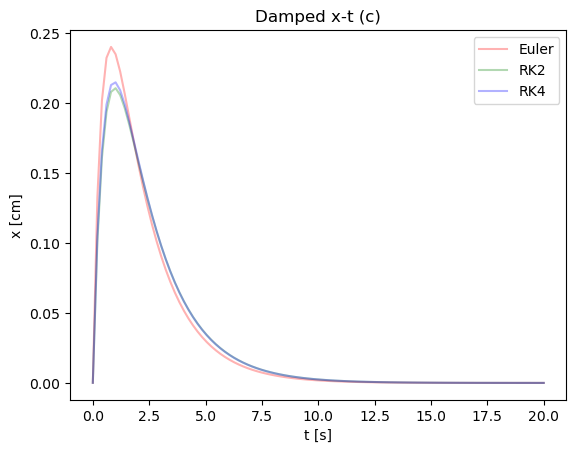
\includegraphics[width = 0.49\textwidth]{damped_c_xt.png}
      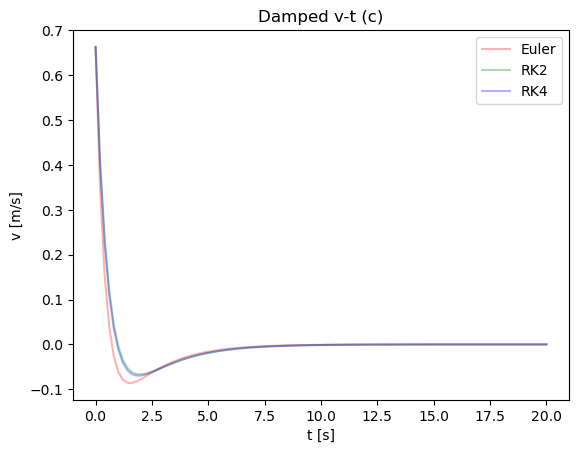
\includegraphics[width = 0.49\textwidth]{damped_c_vt.png}
      \caption{Left is the x-t figure, and right is the v-t. \label{2.c.norm}}
    \end{figure}

    \begin{figure}[H]
        \centering 
        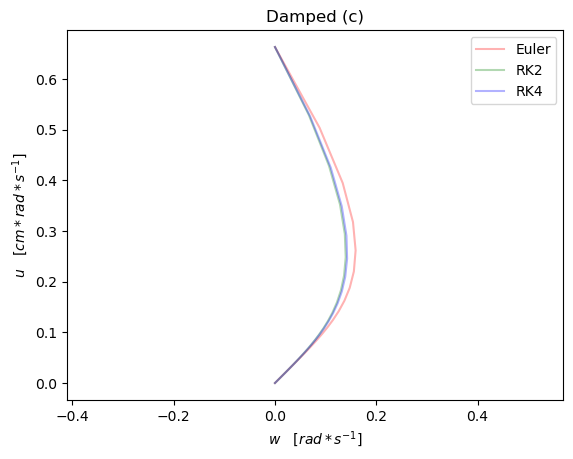
\includegraphics[width = 12cm]{damped_c.png}
        \caption{y-axis is $u$; x-axis is $w$. \label{2.c.pol}}
    \end{figure}

  \subsection{Energy of sec. 2.1.1}
  In this section, we make plots of the total energy and energy loss rate versus time for the underdamped oscillator (a). In Figure \ref{3.a.1}, we can see that the energy is not conserved owing to the dampness; likewise, the loss rate is quick in the beginning and slow in the end since it bases on the velocity, which is correlated to the dampness. On the other hand, we plot the energy difference rate in Figure \ref{3.a.2} as well, showing that the loss rate is not merely oscillating, but also decays along with time.
  \begin{figure}[H]
    \centering 
    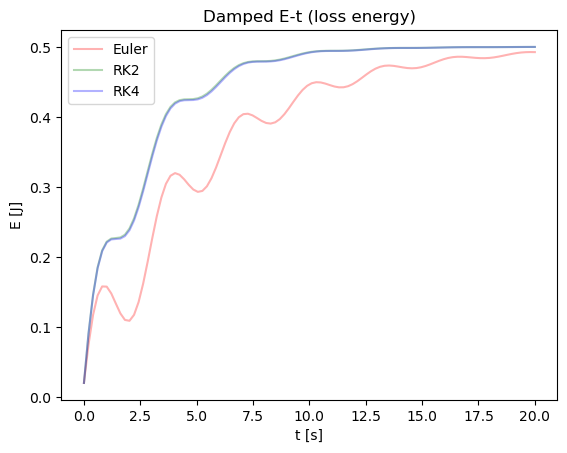
\includegraphics[width = 0.49\textwidth]{damped_a_loss.png}
    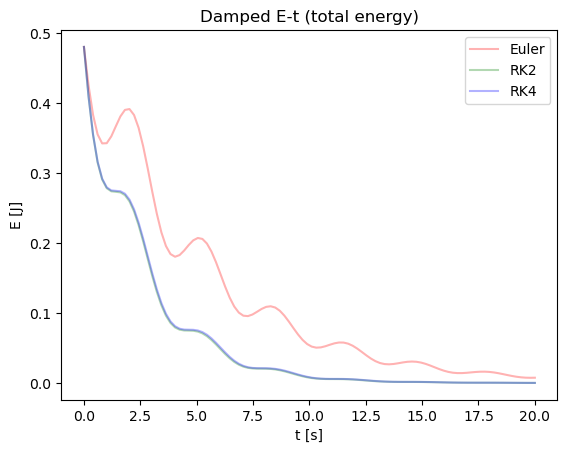
\includegraphics[width = 0.49\textwidth]{damped_a_total.png}
    \caption{Left is the loss energy figure compared with the no-damped model, and right is the total energy depiction. \label{3.a.1}}
  \end{figure}

  \begin{figure}[H]
    \centering 
    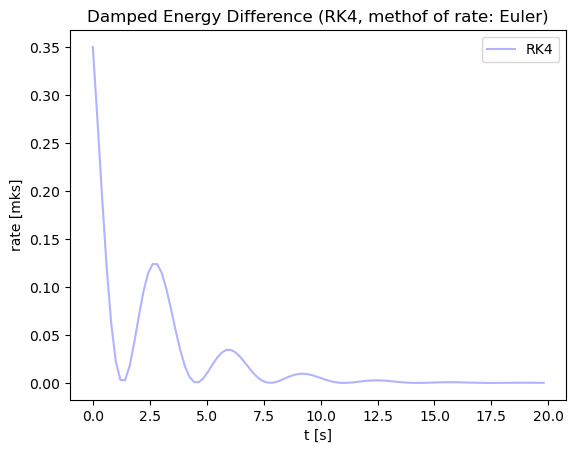
\includegraphics[width = 12cm]{damped_a_rate.png}
    \caption{This is the energy loss rate, utilizing RK4 sample and calculating the rate with Euler method.}
    \label{3.a.2}
  \end{figure}
    
  \subsection{Resonance of forced oscillating}

  In this section, we add a sinusoidal driving force ($F = F_{0} \cos(\omega_{f} t)$) in the damped oscillator with $F_{0} = 0.5$. Vary $\omega_{f}$ from 0.5 to 1.5 with an interval of 0.01 (the question is 0.05, but I think it is too wide). Here, we rerun your simulation up to $t_{max} = 50$, measuring the average amplitude of  oscillator (define $D=<|x(t)|>$ between $40<t<50$). Appling $\lambda = 0.01,\ 0.1,\ 0.3$, we plot these figures in Figure \ref{3}. The resonance appears on $\omega_{f} ~ 1$, and the smaller $\lambda$ the more obvious maximum peak it has.
  \newline
  Theoretically, according to sec. 1.3, the amplitude of forced oscillation is 
  \[\frac{F_{0} / m}{\sqrt{(\omega_0^{2} - \omega_{f}^{2})^{2} + 4\gamma^{2}\omega_{f}^{2}}} = \frac{F_{0} / m}{\sqrt{(\omega_{f}^{2} - \omega_{0}^{2} + 2\gamma^{2})^{2} + 4 \gamma^{2}(\omega_{0}^{2}-\gamma^{2})}}\]
  Thence, when $\omega_{f} = \sqrt{\omega_{0}^{2} - 2 \gamma^{2}} (= \sqrt{\omega_{0}^{2} - \lambda^{2}},\ m = 1)$, the maximum amplitude is 
  \[\frac{F_{0} / m}{2\gamma \sqrt{\omega_{0}^{2} - \gamma^{2}}}\]
  On account of $2\gamma = \lambda / m = \lambda$, and $\omega_{0} = 1$, the maximum (peak) will appear around 1; as $\lambda$ small, it will be more manifest. As a result, compared to the theoretical outcomes, the consequences of the simulation make sense.

  \begin{figure}[H]
    \centering 
    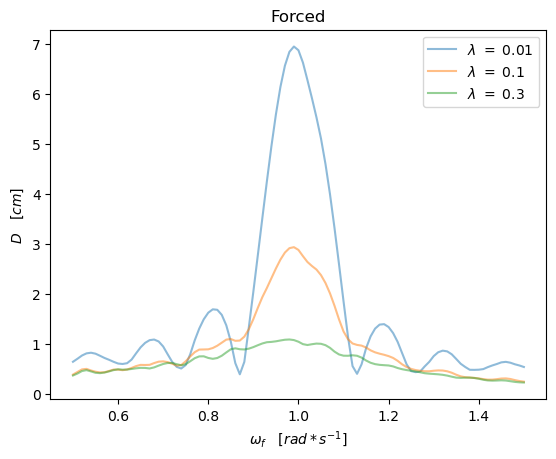
\includegraphics[width = 12cm]{3.png}
    \caption{This is the $D=<|x(t)|>$ vs $\omega_{f}$ between $40<t<50$.\\
            $\lambda = 0.01$, the resonance frequency is on $\omega_f = 0.99$, and the maximum average amplitude is $D = 6.94$.\\
            $\lambda = 0.1$, the resonance frequency is on $\omega_f = 0.99$, and the maximum average amplitude is $D = 2.94$.\\
            $\lambda = 0.3$, the resonance frequency is on $\omega_f = 0.98$, and the maximum average amplitude is $D = 1.09$. \label{3}}
  \end{figure}

  \subsection{RLC circuit systems.}
    \subsubsection{(a) RLC ODE}
    We can apply Kirchoff's rule, which means the current will be conserved or ``the potential(voltage) conservation''.
    \[V_{L} = L\ddot{q},\quad V_{R} = R\dot{q},\quad V_{C} = q/C\]
    and also need to consider the source term, combining that together. We, afterward, can get
    \[L\ddot{q} + R\dot{q} + \frac{q}{C} = E_{0}\sin(\omega t)\quad \blacksquare\]
    Additionally, we can analog RLC system to the forced oscillating system.
      \begin{align*}
        &x \leftrightarrow q,\quad
        \dot{x} \leftrightarrow I,\quad 
        m \leftrightarrow L,\\
        &\lambda \leftrightarrow R,\quad
        1/k \leftrightarrow C,\quad 
        F \leftrightarrow E_{0}
      \end{align*}

    \subsubsection{(b) V-t and I-t}
    Here, we use the conditions
    \[L = C = E_{0} = 1,\quad R = 0.8,\quad \omega = 0.7\]
    Implementing{\ttfamily\ myslover.py} with RK4, we can get the outcomes, as below figures. 

    \begin{figure}[H]
      \centering 
      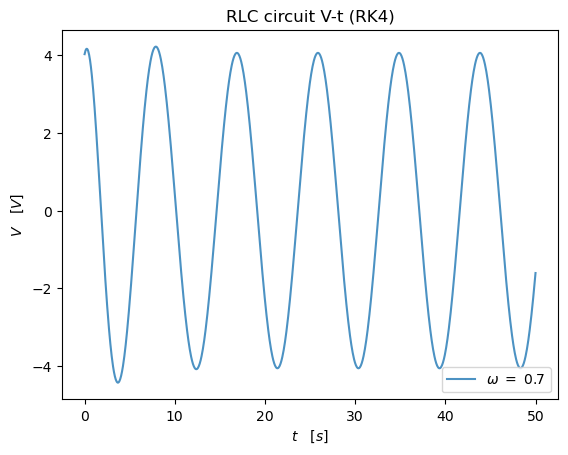
\includegraphics[width = 0.49\textwidth]{4.1.png}
      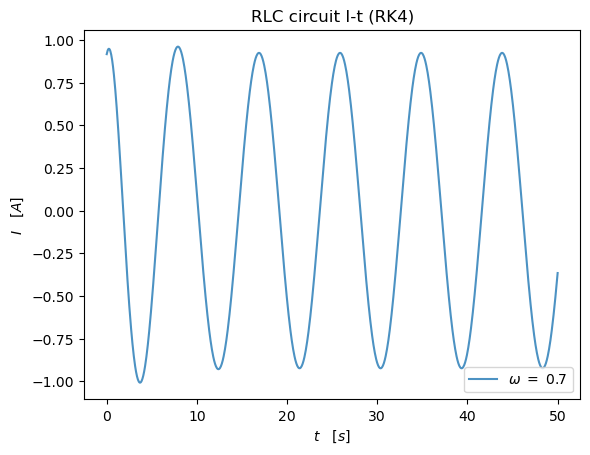
\includegraphics[width = 0.49\textwidth]{4.2.png}
      \caption{Left is the V-t figure, and right is the I-t.}
    \end{figure}

    \subsubsection{(c) Different $\omega$}
    Before utilizing the numerical method, we can calculate theoretical $\omega$s. First is resonance frequency $\omega_{R}$, and another is maximum amplitude frequency $\omega_{M}$, the third is the damped frequency, $\omega_{d}$. (The right approximation corresponds to our varying $\omega$)
      \begin{align*}
        &\omega_{R} = \sqrt{\omega_{0}^{2} - 2\gamma^{2}} \approx 0.8\\
        &\omega_{M} = \frac{1}{LC - R^{2}C^{2}/2} \approx 1.2\qquad [1]\\
        &\omega_{d} = \sqrt{|\omega_{0}^{2} - \gamma^{2}|} \approx 0.9
      \end{align*}

    Referencing the Figure \ref{Compa} and \ref{compa}, from the left V-t figure, we can find that $\omega \approx \omega_{MAX}$, there is a maximum peak, and when $\omega = \omega_{R}$, it shows that the oscillating frequency is approximately equal to the driving frequency; when $\omega < \omega_{d}$ the response of results are greatly ``distort'', compared to the particular solution, and if $\omega > \omega_{d}$, in high frequencies level, it is more likely follow the steady-state solution. All in all, not only the maximum voltage but also the resonance frequency meet our expectations. Besides, we find that the ``transient'' phenomenon still needs to be considered in the low frequencies regime. (Figure \ref{compa}, is the small number of group comparisons)

    \vspace{5cm}

    \footnotesize{[1] Classical Dynamics, 5th edition, page 125, Thornton, Marion}

      \begin{figure}[H]
        \centering 
        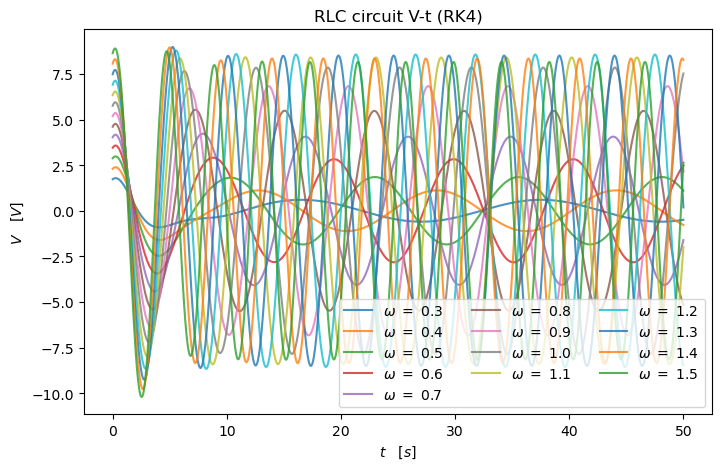
\includegraphics[width = 0.49\textwidth]{4V_tot.png}
        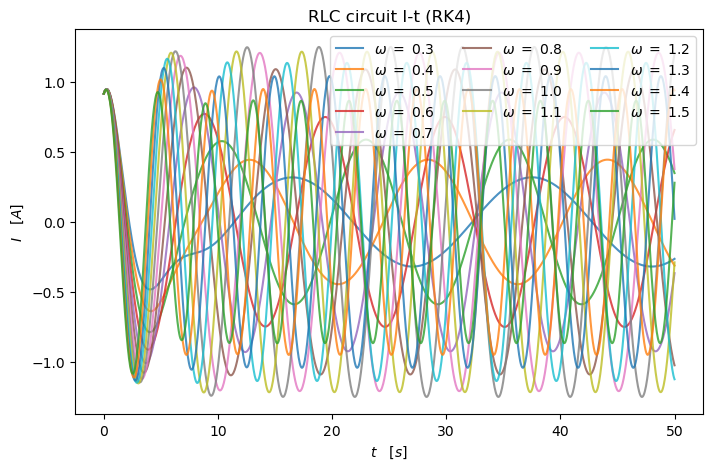
\includegraphics[width = 0.49\textwidth]{4I_tot.png}
        \caption{Left is the V-t figure, and right is the I-t. The plot consists of 13 different frequencies.}
        \label{Compa}
      \end{figure}

      \begin{figure}[H]
        \centering 
        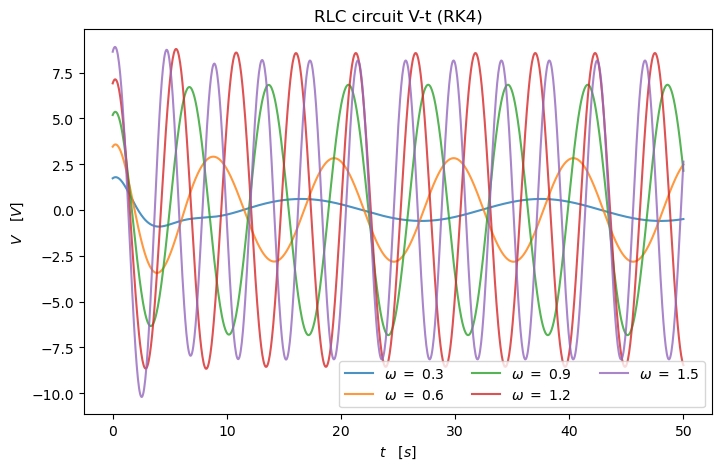
\includegraphics[width = 0.49\textwidth]{V_tot.png}
        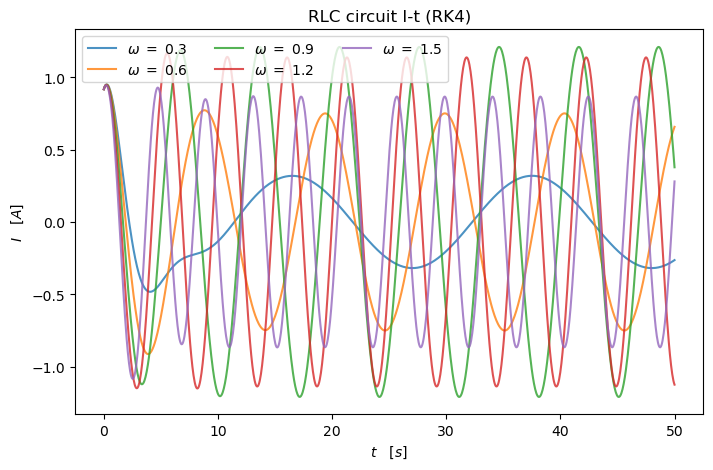
\includegraphics[width = 0.49\textwidth]{I_tot.png}
        \caption{Left is the V-t figure, and right is the I-t. (more concise edition of Figure \ref{Compa})}
        \label{compa}
      \end{figure}

\section{Codes}
    All the codes are transferred from jupyterlab or python codes; hence, if you want to re-run them, please see the source code in the attached files or my GitHub repository: <https://github.com/gary20000915/Comphyslab-HW2.git>.
    \subsection{{\ttfamily\ myslover.py}}
      \begin{lstlisting}[language={Python}]
    """

    This program solves Initial Value Problems (IVP).
    We support three numerical meothds: Euler, Rk2, and Rk4

    Author: Yuan-Yen Peng (edited from Prof. Kuo-Chuan Pan, NTHU 2022.10.06)
    For the course, computational physics lab

    """

    import numpy as np

    def solve_ivp(derive_func, y0, t, dt, N, method, args):
        """
        Solve Initial Value Problems. 

        :param derive_func: a function to describe the derivative of the desired function
        :param y0: an array. The initial state
        :param: t: the instant time of the motion.
        :param dt: the step time
        :param N: the number of steps.
        :param method: string. Numerical method to compute. 
                      We support "Euler", "RK2" and "RK4".
        :param *args: extra arguments for the derive func.

        :return: array_like. solutions. 
        """
        sol_pos, sol_vel = np.array([]), np.array([])
        t = 0
        for _ in range(N):
            t += dt
            sol_pos = np.append(sol_pos, y0[0])
            sol_vel = np.append(sol_vel, y0[1]) 
            y0 = _update(derive_func, y0, t, dt, method, *args)

        return [sol_pos, sol_vel]

    def _update(derive_func, y0, t, dt, method, *args):
        """
        Update the IVP with different numerical method

        :param derive_func: the derivative of the function y'
        :param y0: the initial conditions at time t
        :param: t: the instant time of the motion
        :param dt: the time step dt
        :param method: the numerical method
        :param *args: extral parameters for the derive_func

        :return: the next step condition y0

        """

        if method=="Euler":
            ynext = _update_euler(derive_func,y0, t, dt,*args)
        elif method=="RK2":
            ynext = _update_rk2(derive_func,y0, t, dt,*args)
        elif method=="RK4":
            ynext = _update_rk4(derive_func,y0,t, dt,*args)
        else:
            print("Error: mysolve doesn't supput the method",method)
            quit()
        return ynext

    def _update_euler(derive_func,y0, t, dt,*args):
        """
        Update the IVP with the Euler's method

        :return: the next step solution y

        """
        y0 = np.add(y0, derive_func(y0, t, *args) * dt)

        return y0 # <- change here. just a placeholder

    def _update_rk2(derive_func, y0, t, dt,*args):
        """
        Update the IVP with the RK2 method

        :return: the next step solution y
        """

        k1 = derive_func(y0, t, *args)
        y_temp = y0 + dt * k1 
        k2 = derive_func(y_temp, t, *args) 
        
        y0 = np.add(y0, (dt / 2) * (k1 + k2))
        # note: if use: y0 += (dt / 2) * (k1 + k2) ==> error
        # Yet use y0 = y0 + (dt / 2) * (k1 + k2) ==> it can work, and np.add() can work too.

        return y0 # <- change here. just a placeholder

    def _update_rk4(derive_func,y0, t, dt,*args):
        """
        Update the IVP with the RK4 method

        :return: the next step solution y
        """

        k1 = derive_func(y0, t, *args)
        y_temp = y0 + (dt/2) * k1 # temp for virtual step y*
        k2 = derive_func(y_temp, t, *args)
        y_temp = y0 + (dt/2) * k2
        k3 = derive_func(y_temp, t, *args)
        y_temp = y0 + dt * k3
        k4 = derive_func(y_temp, t, *args)
        
        y0 = np.add(y0, (1/6) * dt * (k1 + 2*k2 + 2*k3 + k4))

        return y0 # <- change here. just a placeholder


    if __name__=='__main__':


        """
        
        Testing mysolver.solve_ivp()

        Kuo-Chuan Pan 2022.10.07

        """


        def oscillator(y,t,K,M):
            '''
            This is the function (osci) defined in the [position, velocity] 
            and [derivative(position), derivative(velocity)]
            :param y: [position, velocity]
            :param k: spring constants
            :param m: mass constant
            '''
            
            yder =  np.zeros(2)
            yder[0] = y[1]
            yder[1] = -y[0] * K/M # the difinition of the acceleration, which is depend on the position.
            print(t) # check to update time
            return yder

        K, M  = 1, 1
        N, t = 100, 20
        dt = t/N
        y0 = np.array([1, 0]) # [pos_0, vel_0]

        sol = solve_ivp(oscillator, y0, t, dt, N, method="RK2", args=(K,M))

        # print("sol=",sol)
        print("Done!")
      \end{lstlisting}

    \subsection{Forced oscillations and RLC circuit}
      \begin{lstlisting}[language={Python}]
      # %% [markdown]
      # 
      # ## Programming Assignment 3 and 4
      # ### 111 Computational Physics Lab  
      #   >Author: Yuan-Yen Peng 108000204  
      #   >Email: garyphys0915@gapp.nthu.edu.com  
      #   >Date: Nov. 11, 2022  
      #   >LINCENCE: MIT

      # %% [markdown]
      # #### 3. Forced oscillator

      # %%
      import numpy as np
      import matplotlib.pyplot as plt
      import mysolver as solver

      # %%
      def oscillator(y,t, lam, wf, F0, K, M):
              '''
              This is the function (osci) defined in the [position, velocity] 
              and [derivative(position), derivative(velocity)]
              :param y: [position, velocity]
              :param t: time (time varying)
              :param lam: \lambda ==> damping constant
              :param wf: \omega_f ==> forceing frequency
              :param F0: initial forceing force
              :param K: spring constants
              :param M: mass constant
              '''
              yder =  np.zeros(2)
              yder[0] = y[1]
              yder[1] = -y[0] * K/M - y[1] * lam / M + F0 * np.cos(wf * t) / M # the difinition of the acceleration, which is depend on the position.

              return yder

      # %%
      def plot(u1, u2, u3, wf, lam):
        '''
        This is the plotting function
        :param ui: u is outcomes. (i = 1, 2, 3) ==> (Euler, RK2, RK4) -> Array
        :param wf: wf is the specified \omega_f. -> Array
        :param lam: the value of lambda. 
        '''
        # plt.plot(wf, u1, "r", alpha = 0.3, label = "Euler")
        # plt.plot(wf, u2, "g", alpha = 0.3, label = "RK2")
        plt.plot(wf, u3, alpha = 0.5, label = f"$\lambda\ =\ {lam}$")
        plt.title(f"Forced")
        plt.ylabel("$D\quad [cm]$")
        plt.xlabel("$\omega_{f}\quad [rad*s^{-1}]$")
        plt.legend(loc = "best")

      # %%
      def CIR_V(t, V, wf):
        '''
        This is the plotting function
        :param t: time. -> Array
        :param V: input voltage. -> Array
        :param wf: wf is the specified \omega_f. -> Array
        '''
        plt.plot(t, V, alpha = 0.8, label = f"$\omega\ =\ {np.round(float(wf), 2)}$")
        plt.title(f"RLC circuit V-t (RK4)")
        plt.ylabel("$V\quad [V]$")
        plt.xlabel("$t\quad [s]$")
        plt.legend(loc = "best", ncol = 3)
        
      def CIR_I(t, I, wf):
        '''
        This is the plotting function
        :param t: time. -> Array
        :param V: input current. -> Array
        :param wf: wf is the specified \omega_f. -> Array
        '''
        plt.plot(t, I, alpha = 0.8, label = f"$\omega\ =\ {np.round(float(wf), 2)}$")
        plt.title(f"RLC circuit I-t (RK4)")
        plt.ylabel("$I\quad [A]$")
        plt.xlabel("$t\quad [s]$")
        plt.legend(loc = "best", ncol = 3)

      # %%
      def para(lam):
        N, t = int(1e3), 50 # divided into 100
        dt = t/N
        T = np.linspace(0, 50, N)

        M, K = 1, 1
        A = 1 # initial amplitude

        phi = - np.pi/2
        r = lam/(2 * M)
        F0 = 0.5
        space = 0.01
        wf = np.arange(0.5, 1.5 + space, space) # [start, stop)
        w0 = np.sqrt(K/M)
        w = np.sqrt(abs(np.square(w0) - np.square(r)))

        y0  = np.zeros(2)
        y0[0]= 0 # initial position
        y0[1] = -A * r * np.cos(phi) - A * w * np.sin(phi)

        # x = np.linspace(0, t, N) # from 0 to t divided by N+1, i.e., N+1 equal parts.

        ind = np.where(T >= 40)
        RANGE = np.array([ind])

        D1 = np.zeros(len(wf))
        D2 = np.zeros(len(wf))
        D3 = np.zeros(len(wf))

        for i in range(len(wf)):
          sol1 = solver.solve_ivp(oscillator, y0, t, dt, N, method="Euler", args=(lam, wf[i], F0, K, M))[0]
          D1[i] = np.average(np.abs(sol1[RANGE]))
          sol2 = solver.solve_ivp(oscillator, y0, t, dt, N, method="RK2", args=(lam, wf[i], F0, K, M))[0]
          D2[i] = np.average(np.abs(sol2[RANGE]))
          sol3 = solver.solve_ivp(oscillator, y0, t, dt, N, method="RK4", args=(lam, wf[i], F0, K, M))[0]
          D3[i] = np.average(np.abs(sol3[RANGE]))

        D3_MAX_ind = np.where(D3 == np.max(D3))
        wf_MAX = float(wf[D3_MAX_ind])
        print(f"When \lambda = {lam}, the resonance frequency is on \omega_f = {wf_MAX}, and the average amplitude is D = {float(np.max(D3))}.")
        
        return D1, D2, D3, wf, lam

      # %%
      out = para(0.01)
      plot(out[0], out[1], out[2], out[3], out[4])
      out = para(0.1)
      plot(out[0], out[1], out[2], out[3], out[4])
      out = para(0.3)
      plot(out[0], out[1], out[2], out[3], out[4])

      # %% [markdown]
      # #### 4. RLC circuit

      # %%
      def RLC(y, t, L, R, C, wf, E0):
              '''
              This is the function (osci) defined in the [position, velocity] 
              and [derivative(position), derivative(velocity)]
              :param y: [position, velocity]
              :param t: time (time varying)
              :param lam: \lambda ==> damping constant
              :param wf: \omega_f ==> forceing frequency
              :param F0: initial forceing force
              :param K: spring constants
              :param M: mass constant
              '''
              yder =  np.zeros(2)
              yder[0] = y[1]
              yder[1] = -y[0] / (C * L) - y[1] * R / L + E0 * np.cos(wf * t) / L # the difinition of the acceleration, which is depend on the position.

              return yder

      # %%

      N, t = int(1e3), 50 # divided into 100
      dt = t/N
      T = np.linspace(0, 50, N)

      L, C = 1, 1
      A = 1 # initial amplitude
      phi = - np.pi/2

      R = 0.8
      r = R / (2 * L)
      E0 = 1
      # space = 0.1
      # wf = np.arange(0.3, 1.5 + space, space) # [start, stop)
      wf = np.array([0.7])
      w0 = np.sqrt(1 / (C * L))
      w = np.sqrt(abs(np.square(w0) - np.square(r)))

      y0  = np.zeros(2)
      y0[0]= 0 # initial position
      y0[1] = -A * r * np.cos(phi) - A * w * np.sin(phi)

      # x = np.linspace(0, t, N) # from 0 to t divided by N+1, i.e., N+1 equal parts.

      for i in range(len(wf)):
        X_L = 2 * np.pi * wf[i] * L
        I1 = solver.solve_ivp(RLC, y0, t, dt, N, method="Euler", args=(L, R, C, wf[i], E0))[1]
        V1 = I1 * X_L
        I2 = solver.solve_ivp(RLC, y0, t, dt, N, method="RK2", args=(L, R, C, wf[i], E0))[1]
        V2 = I2 * X_L
        I3 = solver.solve_ivp(RLC, y0, t, dt, N, method="RK4", args=(L, R, C, wf[i], E0))[1]
        V3 = I3 * X_L
        CIR_V(T, V3, wf[i])
        plt.show()
        CIR_I(T, I3, wf[i])
        plt.show()

      # %%
      N, t = int(1e3), 50 # divided into 100
      dt = t/N
      T = np.linspace(0, t, N)

      L, C = 1, 1
      A = 1 # initial amplitude
      phi = - np.pi/2

      R = 0.8
      r = R / (2 * L)
      E0 = 1
      space = 0.1
      wf = np.arange(0.3, 1.5 + space, space) # [start, stop)
      # wf = np.array([0.7])
      w0 = np.sqrt(1 / (C * L))
      w = np.sqrt(abs(np.square(w0) - np.square(r)))

      y0  = np.zeros(2)
      y0[0]= 0 # initial position
      y0[1] = -A * r * np.cos(phi) - A * w * np.sin(phi)

      print(np.sqrt(w0 ** 2 - 2 * r ** 2))
      print(1/np.sqrt(L*C - 0.5 * (R*C) ** 2))
      print(w)
      # x = np.linspace(0, t, N) # from 0 to t divided by N+1, i.e., N+1 equal parts.

      plt.figure(figsize = (8.1,5))
      for i in range(len(wf)):
        X_L =  2 * np.pi * wf[i] * L
        I1 = solver.solve_ivp(RLC, y0, t, dt, N, method="Euler", args=(L, R, C, wf[i], E0))[1]
        V1 = I1 * X_L
        I2 = solver.solve_ivp(RLC, y0, t, dt, N, method="RK2", args=(L, R, C, wf[i], E0))[1]
        V2 = I2 * X_L
        I3 = solver.solve_ivp(RLC, y0, t, dt, N, method="RK4", args=(L, R, C, wf[i], E0))[1]
        V3 = I3 * X_L
        CIR_I(T, I3, wf[i])
        
      plt.figure(figsize = (8.1,5))
      for i in range(len(wf)):
        X_L =  2 * np.pi * wf[i] * L
        I1 = solver.solve_ivp(RLC, y0, t, dt, N, method="Euler", args=(L, R, C, wf[i], E0))[1]
        V1 = I1 * X_L
        I2 = solver.solve_ivp(RLC, y0, t, dt, N, method="RK2", args=(L, R, C, wf[i], E0))[1]
        V2 = I2 * X_L
        I3 = solver.solve_ivp(RLC, y0, t, dt, N, method="RK4", args=(L, R, C, wf[i], E0))[1]
        V3 = I3 * X_L
        CIR_V(T, V3, wf[i])

      # %%
      plt.figure(figsize = (8.1,5))
      for i in range(0, len(wf), 3):
        X_L =  2 * np.pi * wf[i] * L
        I3 = solver.solve_ivp(RLC, y0, t, dt, N, method="RK4", args=(L, R, C, wf[i], E0))[1]
        V3 = I3 * X_L
        CIR_V(T, V3, wf[i])

      # %%
      plt.figure(figsize = (8.1,5))
      for i in range(0, len(wf), 3):
        X_L =  2 * np.pi * wf[i] * L
        I3 = solver.solve_ivp(RLC, y0, t, dt, N, method="RK4", args=(L, R, C, wf[i], E0))[1]
        V3 = I3 * X_L
        CIR_I(T, I3, wf[i])

      # %%
      \end{lstlisting}

    \subsection{Damped Oscillator}
      \begin{lstlisting}[language={Python}]
      # %% [markdown]
      # 
      # ## Programming Assignment 1 and 2
      # ### 111 Computational Physics Lab  
      #   >Author: Yuan-Yen Peng 108000204  
      #   >Email: garyphys0915@gapp.nthu.edu.com  
      #   >Date: Nov. 11, 2022  
      #   >LINCENCE: MIT

      # %% [markdown]
      # #### 1. Damped oscillator

      # %%
      import numpy as np
      import matplotlib.pyplot as plt
      import mysolver as solver

      # %%
      def oscillator(y,t, lam, K, M):
              '''
              This is the function (osci) defined in the [position, velocity] 
              and [derivative(position), derivative(velocity)]
              :param y: [position, velocity]
              :param t: time (time varying)
              :param lam: \lambda ==> damping constant
              :param K: spring constants
              :param M: mass constant
              '''
              yder =  np.zeros(2)
              yder[0] = y[1]
              yder[1] = -y[0] * K/M - y[1] * lam / M # the difinition of the acceleration, omghich is depend on the position.
              
              return yder

      # %%
      def plot(u1, u2, u3, w1, w2, w3, num):
        '''
        This is the plotting function
        :param ui: u is the specified polared unit for x-axis. (i = 1, 2, 3) ==> (Euler, RK2, RK4)
        :param wi: w is the specified polared unit for y-axis. (i = 1, 2, 3) ==> (Euler, RK2, RK4)
        '''
        plt.plot(u1, w1, "r", alpha = 0.3, label = "Euler")
        plt.plot(u2, w2, "g", alpha = 0.3, label = "RK2")
        plt.plot(u3, w3, "b", alpha = 0.3, label = "RK4")
        plt.axis("equal")
        plt.title(f"Damped ({num})")
        plt.xlabel("$w\quad [rad*s^{-1}]$")
        plt.ylabel("$u\quad [cm*rad*s^{-1}]$")
        plt.legend(loc = "best")
        plt.show()

      # %%
      def xt(t_eval, sol1, sol2, sol3, sub):
        plt.plot(t_eval, sol1, "r", label = "Euler", alpha = 0.3)
        plt.plot(t_eval, sol2, "g", label = "RK2", alpha = 0.3)
        plt.plot(t_eval, sol3, "b", label = "RK4", alpha = 0.3)
        plt.title(f"Damped x-t ({sub})")
        plt.xlabel("t [s]")
        plt.ylabel("x [cm]")
        plt.legend()
        plt.show()
        
      def vt(t_eval, sol1, sol2, sol3, sub):
        plt.plot(t_eval, sol1, "r", label = "Euler", alpha = 0.3)
        plt.plot(t_eval, sol2, "g", label = "RK2", alpha = 0.3)
        plt.plot(t_eval, sol3, "b", label = "RK4", alpha = 0.3)
        plt.title(f"Damped v-t ({sub})")
        plt.xlabel("t [s]")
        plt.ylabel("v [m/s]")
        plt.legend()
        plt.show()

      # %%
      def et(t_eval, sol1, sol2, sol3, sub):
        plt.plot(t_eval, sol1, "r", label = "Euler", alpha = 0.3)
        plt.plot(t_eval, sol2, "g", label = "RK2", alpha = 0.3)
        plt.plot(t_eval, sol3, "b", label = "RK4", alpha = 0.3)
        plt.title(f"Damped E-t ({sub})")
        plt.xlabel("t [s]")
        plt.ylabel("E [J]")
        plt.legend()
        plt.show()

      # %%
      def rate(t_eval, sol1, sol2, sol3, sub):
        # plt.plot(t_eval, sol1, "r", label = "Euler", alpha = 0.3)
        # plt.plot(t_eval, sol2, "g", label = "RK2", alpha = 0.3)
        plt.plot(t_eval, sol3, "b", label = "RK4", alpha = 0.3)
        plt.title(f"Damped Energy Difference ({sub})")
        plt.xlabel("t [s]")
        plt.ylabel("rate [mks]")
        plt.legend()
        plt.show()

      # %% [markdown]
      # (a) $A = 1 [cm],\quad \omega_0 = 1 [rads^{-1}],\quad \gamma = 0.2 [s^{-1}], \quad \phi = -\pi / 2 [rad]$

      # %%
      # Setting parameters
      N, t = 100, 20
      dt = t/N

      M, K = 1, 1
      A = 1 # initial amplitude
      r  = 0.2 # \gamma
      lam = 2 * M * r # \lamda
      phi = - np.pi/2
      omg0 = np.sqrt(K/M)
      omg1 = np.sqrt(abs(np.square(omg0) - np.square(r)))

      y0  = np.zeros(2)
      y0[0]= 0 # initial position
      y0[1] = - A * r * np.cos(phi) - A * omg1 * np.sin(phi) # initial velocity

      t_eval = np.linspace(0, t, N) # from 0 to t divided by N+1, i.e., N+1 equal parts.

      # %%
      # position
      sol1 = solver.solve_ivp(oscillator, y0, t, dt, N, method="Euler", args=(lam, K, M))[0]
      sol2 = solver.solve_ivp(oscillator, y0, t, dt, N, method="RK2", args=(lam, K, M))[0]
      sol3 = solver.solve_ivp(oscillator, y0, t, dt, N, method="RK4", args=(lam, K, M))[0]

      # velocity
      sol1_v = solver.solve_ivp(oscillator, y0, t, dt, N, method="Euler", args=(lam, K, M))[1]
      sol2_v = solver.solve_ivp(oscillator, y0, t, dt, N, method="RK2", args=(lam, K, M))[1]
      sol3_v = solver.solve_ivp(oscillator, y0, t, dt, N, method="RK4", args=(lam, K, M))[1]

      # %%
      # Visualize
      xt(t_eval, sol1, sol2, sol3, "a")
      vt(t_eval, sol1_v, sol2_v, sol3_v, "a")

      # %%
      # polar coordinates
      u1 = omg1 * sol1
      u2 = omg1 * sol2
      u3 = omg1 * sol3

      w1 = r * sol1 + sol1_v
      w2 = r * sol2 + sol2_v
      w3 = r * sol3 + sol3_v

      # plot it!
      plot(u1, u2, u3, w1, w2, w3, "a")

      # %% [markdown]
      # #### 2. Total energy and the energy loss

      # %%
      # kenetical energy
      K1 = 0.5 * M * np.square(sol1)
      K2 = 0.5 * M * np.square(sol2)
      K3 = 0.5 * M * np.square(sol3)

      # potential energy
      U1 = 0.5 * K * np.square(sol1_v)
      U2 = 0.5 * K * np.square(sol2_v)
      U3 = 0.5 * K * np.square(sol3_v)

      # total energy
      tot1 = K1 + U1
      tot2 = K2 + U2
      tot3 = K3 + U3

      # energy loss
      no_loss = 0.5 * K * np.square(A)
      loss1 = no_loss - tot1
      loss2 = no_loss - tot2
      loss3 = no_loss - tot3

      # rate of energy loss
      rate3 = np.array([])
      for i in range (len(loss3) - 1):
          rate3 = np.append(rate3, (loss3[i+1] - loss3[i]) / dt)

      rate2 = (loss2 / no_loss) * 100
      rate1 = (loss1 / no_loss) * 100

      # plot them!
      et(t_eval, tot1, tot2, tot3, "total energy")
      et(t_eval, loss1, loss2, loss3, "loss energy")
      t_eval_prime = t_eval[0:-1]
      rate(t_eval_prime, rate1, rate2, rate3, "RK4, methof of rate: Euler")


      # %% [markdown]
      # ### 1. (conti)
      # (b) $A = 1 [cm],\quad \omega_0 = 1 [rads^{-1}],\quad \gamma = 1.0 [s^{-1}], \quad \phi = -\pi / 2 [rad]$

      # %%
      # update the parameter \gamma
      # Setting parameters
      N, t = 100, 20
      dt = t/N

      M, K = 1, 1
      A = 1 # initial amplitude
      r  = 1.0 # \gamma
      lam = 2 * M * r # \lamda
      phi = - np.pi/2
      omg0 = np.sqrt(K/M)
      omg1 = np.sqrt(abs(np.square(omg0) - np.square(r)))

      y0  = np.zeros(2)
      y0[0]= 10e-5 # initial position (use tolerence = 10e-5)
      y0[1] = - A * r * np.cos(phi) - A * omg1 * np.sin(phi) # initial velocity

      t_eval = np.linspace(0, t, N) # from 0 to t divided by N+1, i.e., N+1 equal parts.

      # %%
      # position
      sol1 = solver.solve_ivp(oscillator, y0, t, dt, N, method="Euler", args=(lam, K, M))[0]
      sol2 = solver.solve_ivp(oscillator, y0, t, dt, N, method="RK2", args=(lam, K, M))[0]
      sol3 = solver.solve_ivp(oscillator, y0, t, dt, N, method="RK4", args=(lam, K, M))[0]

      # velocity
      sol1_v = solver.solve_ivp(oscillator, y0, t, dt, N, method="Euler", args=(lam, K, M))[1]
      sol2_v = solver.solve_ivp(oscillator, y0, t, dt, N, method="RK2", args=(lam, K, M))[1]
      sol3_v = solver.solve_ivp(oscillator, y0, t, dt, N, method="RK4", args=(lam, K, M))[1]

      # %%
      # Visualize
      xt(t_eval, sol1, sol2, sol3, "b")
      vt(t_eval, sol1_v, sol2_v, sol3_v, "b")

      # %%
      # polar coordinates
      u1 = omg1 * sol1
      u2 = omg1 * sol2
      u3 = omg1 * sol3

      w1 = r * sol1 + sol1_v
      w2 = r * sol2 + sol2_v
      w3 = r * sol3 + sol3_v

      # plot it!
      plot(u1, u2, u3, w1, w2, w3, "b")

      # %% [markdown]
      # (c) $A = 1 [cm],\quad \omega_0 = 1 [rads^{-1}],\quad \gamma = 1.2 [s^{-1}], \quad \phi = -\pi / 2 [rad]$

      # %%
      # update the parameter \gamma
      # Setting parameters
      N, t = 100, 20
      dt = t/N

      M, K = 1, 1
      A = 1 # initial amplitude
      r  = 1.2 # \gamma
      lam = 2 * M * r # \lamda
      phi = - np.pi/2
      omg0 = np.sqrt(K/M)
      omg1 = np.sqrt(abs(np.square(omg0) - np.square(r)))

      y0  = np.zeros(2)
      y0[0]= 0 # initial position (use tolerence = 10e-5)
      y0[1] = - A * r * np.cos(phi) - A * omg1 * np.sin(phi) # initial velocity

      t_eval = np.linspace(0, t, N) # from 0 to t divided by N+1, i.e., N+1 equal parts.

      # %%
      # position
      sol1 = solver.solve_ivp(oscillator, y0, t, dt, N, method="Euler", args=(lam, K, M))[0]
      sol2 = solver.solve_ivp(oscillator, y0, t, dt, N, method="RK2", args=(lam, K, M))[0]
      sol3 = solver.solve_ivp(oscillator, y0, t, dt, N, method="RK4", args=(lam, K, M))[0]

      # velocity
      sol1_v = solver.solve_ivp(oscillator, y0, t, dt, N, method="Euler", args=(lam, K, M))[1]
      sol2_v = solver.solve_ivp(oscillator, y0, t, dt, N, method="RK2", args=(lam, K, M))[1]
      sol3_v = solver.solve_ivp(oscillator, y0, t, dt, N, method="RK4", args=(lam, K, M))[1]

      # %%
      # Visualize
      xt(t_eval, sol1, sol2, sol3, "c")
      vt(t_eval, sol1_v, sol2_v, sol3_v, "c")

      # %%
      # polar coordinates
      u1 = omg1 * sol1
      u2 = omg1 * sol2
      u3 = omg1 * sol3

      w1 = r * sol1 + sol1_v
      w2 = r * sol2 + sol2_v
      w3 = r * sol3 + sol3_v

      # plot it!
      plot(u1, u2, u3, w1, w2, w3, "c")
      \end{lstlisting}
      
\end{document}